\documentclass{article}
\usepackage{amsmath,amssymb,amsfonts}   % For math symbols and fonts
\usepackage{graphicx}                   % For including images
\usepackage{hyperref}                   % For hyperlinks
\usepackage{cite}                       % For citations
\usepackage[utf8]{inputenc}             % For UTF-8 encoding

\usepackage{algorithm}
\usepackage{algorithmic}

\usepackage{amsthm}
% Define new theorem-like environments
\newtheorem{definition}{Definition}[section]    % Definition environment
\newtheorem{theorem}{Theorem}[section]          % Theorem environment
\newtheorem{exercise}{Exercise}[section]        % Exercise environment


% Title and author info
\title{Separation Axioms Summary}
\author{Zhang Jinrui\thanks{alternative email:jerryzhang40@gmail.com} \\ \texttt{zhangjr1022@mails.jlu.edu.cn}}

\date{20241120}  % Empty date; optional, you can also specify a date here

\begin{document}

\maketitle

\begin{abstract}
    In this short essay I summarised the separation Axioms I have
    leared, in the topology course. Argued the subspace hereditary,
    productspace hereditary, and the Continuity-preserving property.
    And slightly discuss the relationships between these Axioms.
\end{abstract}


\section{Motivation of Separation Axioms}
The basic Axioms of topology only described the relationship of the
opensets, the opensets captured the geometry structure in the point set.
but it some of the coarse topology dose not have a much resonable
behavior, such as the indiscrete topology, even the const sequence
could converge to any point in the base set. this is because the
topology is so coarse that we only have two opensets that is $\{\phi, X\}$
so all the structure we care is crushed together in this topology.

The Separation Axioms served as patched to the basic Axioms of topology
to make sure we are deal with some topology space with some familiar
behaviors. This is the motivation and mean of Introduction these
Axioms patches.\cite[script1]{MAT327topology1script}

\section{All the Axioms}
\subsection{Definition of Separation Axioms}
First lets see three basic separation concepts,
that is Hausdorff, regular and normal.
Figure\ref{fig:regular} has well illustrated the
idea.
\begin{definition}[regular]
    A topological space X is a regular space if,
    given any closed set F and any point x that
    does not belong to F, there exists a neighbourhood
    U of x and a neighbourhood V of F
    that are disjoint. Concisely put,
    it must be possible to separate x and F
    with disjoint neighborhoods.
    \cite[Reglarspace]{Reglarspace}
    Figure\ref{fig:regular}
\end{definition}
\begin{definition}[normal]
    A topological space X is a normal space if, given
    any disjoint closed sets E and F, there are
    neighbourhoods U of E and V of F that are also
    disjoint. More intuitively, this condition says
    that E and F can be separated by neighbourhoods.
    \cite[Normal]{Normal}
    % Figure\ref{fig:regular}
\end{definition}
\begin{definition}[closed neighborhoods separation]
    We say that x and y can be separated by closed
    neighborhoods if there exists a closed neighborhood
    U of x and a closed neighborhood V of y such that U
    and V are disjoint $(U \cap V = \emptyset)$.
    (Note that a "closed neighborhood of x" is
    a closed set that contains an open set
    containing x.)
    \cite[UandcHs]{UandcHs}
\end{definition}
Another important concept is completeness.
The prefix "completely" add ahead the
Hausdorff, regular and normal neams the
corresponding two object can be separate
by functions.
\begin{definition}[continuous separation]
    We say that x and y can be separated by a function
    if there exists a continuous function
    $f:X \to [0,1]$ (the unit interval) with
    $f(x) = 0$ and $f(y) = 1$.
    \cite[UandcHs]{UandcHs}
\end{definition}
\begin{definition}[set separate by function]
    We say that two sets X and Y can
    be separated by a function
    if there exists a continuous function
    $f:X \to [0,1]$ (the unit interval) with
    $f\vert _{X} = 0$ and $\vert _{Y} = 1$.
    \cite[UandcHs]{UandcHs}
\end{definition}
\begin{definition}[completely regular]
    A topological space
    X is called completely regular if points can be
    separated from closed sets via (bounded) continuous real-valued functions. In technical terms this means: for any closed set
    ${\displaystyle A\subseteq X}$ and any point,
    ${\displaystyle x\in X\setminus A,}$ there
    exists a real-valued continuous function
    ${\displaystyle f:X\to \mathbb {R} }$ such that
    ${\displaystyle f(x)=1}$ and
    ${\displaystyle f\vert _{A}=0.}$ \
    (Equivalently one can choose any two values
    instead of
    ${\displaystyle 0}$ and
    ${\displaystyle 1}$ and even require that
    ${\displaystyle f}$ be a bounded function.)
    \cite[Tychonoff]{Tychonoff}
\end{definition}
The following part is all the $T$ Axioms.
\begin{definition}[$T_0$]
    A topological space $(X, \mathcal{T})$ is said to be $T_0$ (or much less commonly said to
    be a Kolmogorov space), if for any pair of distinct points $x, y \in X$ there is an open set U that
    contains one of them and not the other.
    \cite[script5]{MAT327topology5script}
\end{definition}
\begin{definition}[$T_1$]
    A topological space $(X, \mathcal{T})$ is said to be $T_1$ (or much less commonly said to be
    a Fr\'echet space) if for any pair of distinct points $x, y \in X$, there exist open sets U and V such
    that U contains x but not y, and V contains y but not x.
    \cite[script5]{MAT327topology5script}
\end{definition}
\begin{definition}[$T_2$]
    A topological space $(X, \mathcal{T})$ is said to be $T_2$, or more commonly said to be
    a Hausdorff space, if for every pair of distinct points $x, y \in X$, there exist disjoint open sets $U$
    and $V$ such that $x \in U$ and $y \in V$.
    \cite[script5]{MAT327topology5script}
\end{definition}
\begin{theorem}
    Let $(X, \mathcal{T})$ be a Hausdorff space. Then every sequence in $X$
    converges to at most one point.
    \cite[script5]{MAT327topology5script}
\end{theorem}
$Proof.$ Suppose $X$ is Hausdorff and let ${x_n}$ be a sequence in $X$. Suppose $x_n \to x$ and $y \not= x$.
Then there are disjoint open sets $U$ and $V$ such that $x \in U$ and $y \in V$ . By definition of
convergence, some tail of the sequence is in the set U. But then that tail (and therefore all tails
of the sequence) is disjoint from $V$ , meaning $x_n \not\to y$.\cite[script5]{MAT327topology5script}
\begin{definition}[$T_{2\frac{1}{2}}$]
    A Urysohn space, also called a $T_{2\frac{1}{2}}$
    space, is a space in which any two distinct points
    can be separated by closed neighborhoods.
    \cite[UandcHs]{UandcHs}
\end{definition}
\begin{definition}[completely $T_2$]
    A completely Hausdorff space, or completely $T_2$,
    or functionally
    Hausdorff space, is a space in which any two
    distinct points can be separated by a continuous
    function.
    \cite[UandcHs]{UandcHs}
\end{definition}
\begin{definition}[$T_3$]
    A $T_3$ space or regular Hausdorff space is a
    topological space that is both regular and a
    Hausdorff space.
    \cite[Reglarspace]{Reglarspace}
\end{definition}
\begin{definition}[$T_{3\frac{1}{2}}$]
    A topological space is called a
    Tychonoff space (alternatively:
    $T_{3\frac{1}{2}}$ space, or $T_\pi$ space,
    or completely
    $T_3$ space) if it is a
    completely regular Hausdorff space.
    \cite[Tychonoff]{Tychonoff}
\end{definition}
\begin{definition}[$T_4$]
    A T4 space is a $T_1$ space X that is normal;
    this is equivalent to X being normal and
    Hausdorff.
    \cite[Tychonoff]{Tychonoff}
\end{definition}
\begin{definition}[$T_5$]
    A $T_5$ space, or completely $T_4$ space,
    is a completely normal $T_1$ space X,
    which implies that X is Hausdorff;
    equivalently, every subspace of X
    must be a $T_4$ space.
    \cite[Tychonoff]{Tychonoff}
\end{definition}
\begin{definition}[$T_6$]
    A $T_6$ space, or perfectly $T_4$ space,
    is a perfectly normal Hausdorff space.
    \cite[Tychonoff]{Tychonoff}
\end{definition}

\subsection{Some properties}
\begin{theorem}[$T_0$ hereditary]
    If a space is $T_0$ then its subspace is
    also $T_0$
\end{theorem}
$Proof.$ The subspace presere the open sets
of the original space. The definition of the
$T_0$ space only contains the definition
of the open sets.

Suppose $x,y\in E\subset X$ then
$\exists U\in \mathcal{T}$
that $x\in U, y \not\in U$
then $U_E = E \cap U \in \mathcal{T}_E$
that $x\in U_E, y \not\in U_E$

\begin{theorem}[$T_0$ productspace]
    If a space is $T_0$ then its productspace is
    also $T_0$
\end{theorem}
$Proof.$ The productspace also can
presere the open sets
of the original space.

Suppose $(X,\mathcal{T}_X),(Y,\mathcal{T}_Y)$ are
$T_0$ space.
then the product space
$(P,\mathcal{T}_P)
    =
    (X\times Y, \mathcal{T}_X\times\mathcal{T}_Y)$
if two points
$(x,y)\not=(x',y')\in P$
then there at least one coordinate are distinct
Suppose $x\not=x'$ then
$\exists U\in \mathcal{T_X}$
that $x\in U, x' \not\in U$
then
$\exists U_P=U\times Y\in \mathcal{T_P}$
that
that $x\in U_P, x' \not\in U_P$

For the continuous image $X\to Y$.
We can just let $(Y,\mathcal{T}_{trivial})$
then any Separation Axioms would not presere
in the image $f(X)\subset Y$

\subsection{Examples and counterExamples}
Spaces that are not $T_0$

A set with more than one element, with the trivial topology. No points are distinguishable.

The set R2 where the open sets are the Cartesian product of an open set in R and R itself, i.e., the product topology of R with the usual topology and R with the trivial topology; points (a,b) and (a,c) are not distinguishable.

The space of all measurable functions f from the real line R to the complex plane C such that the Lebesgue integral
${\displaystyle \left(\int _{\mathbb {R} }|f(x)|^{2}\,dx\right)^{\frac {1}{2}}<\infty }$. Two functions which are equal almost everywhere are indistinguishable. See also below.

Spaces that are $T_0$ but not $T_1$

The Zariski topology on Spec(R), the prime spectrum of a commutative ring R, is always $T_0$ but generally not $T_1$. The non-closed points correspond to prime ideals which are not maximal. They are important to the understanding of schemes.

The particular point topology on any set with at least two elements is $T_0$ but not $T_1$ since the particular point is not closed (its closure is the whole space). An important special case is the Sierpiński space which is the particular point topology on the set {0,1}.

The excluded point topology on any set with at least two elements is $T_0$ but not $T_1$. The only closed point is the excluded point.

The Alexandrov topology on a partially ordered set is $T_0$ but will not be $T_1$ unless the order is discrete (agrees with equality). Every finite $T_0$ space is of this type. This also includes the particular point and excluded point topologies as special cases.

The right order topology on a totally ordered set is a related example.

The overlapping interval topology is similar to the particular point topology since every non-empty open set includes 0.

Quite generally, a topological space X will be $T_0$ if and only if the specialization preorder on X is a partial order. However, X will be $T_1$ if and only if the order is discrete (i.e. agrees with equality). So a space will be $T_0$ but not $T_1$ if and only if the specialization preorder on X is a non-discrete partial order.
\subsection{Relationship between Separation Axioms}
$
    T_6
    \Rightarrow T_5
    \Rightarrow T_4
    \Rightarrow T_{3\frac{1}{2}}
    \Rightarrow T_3
    \Rightarrow T_{2\frac{1}{2}}
    \Rightarrow T_2
    \Rightarrow T_1
    \Rightarrow T_0
$

Each implication is strict


% \section{Results}
% \subsection{first approach}
% Train the model on a pure $sin(x)$ and try to
% get a result that satisfies the initial condition with
% $U^{t}_0=0.5$ and $U_0=0.0$ to which the exact solution is $0.5*sin(x)$ would. The result is shown in Figure\ref{fig:fig1}.
% \subsection{approach with linear assumption}
% Train the model on a pure $sin(x)$ and try to
% get a result that satisfies the initial condition with
% $U^{t}_0=0.5$ and $U_0=0.5$ in which the exact solution is $\frac{\sqrt{2}}{2}*sin(x+\frac{\pi}{4})$ would be
% required output. The result is shown in Figure\ref{fig:fig2}.
% \subsection{approach augmentation}
% Train the model on a 2D circle and try to
% get a result of $x^\delta=y^\delta(\rho)=[cos(\rho),sin(\rho)]$,
% and the corresponding differential equation is
% $\frac{\partial^2 y_\delta}{{\partial \rho}^2}+y_\delta=0$
% Result of the latent space structure shows in Figures\ref{fig:fig3} and Figure\ref{fig:fig4}, with the
% numerical result $0.7360\frac{\partial^2 y_\delta}{{\partial \rho}^2}-0.0328\frac{\partial y_\delta}{{\partial \rho}}+  0.6761y_\delta=0$.

% \begin{figure}[h!]
%     \centering
%     \includegraphics[width=0.45\textwidth]{figde3/draw_2D__GeneredData.png}
%     \includegraphics[width=0.5\textwidth]{figde3/draw_2D__GeneredEqu.png}
%     \caption{generated data using the PINN to get $0.5*sin(x)$}
% \end{figure}
\begin{figure}[ht!]
    \centering
    \begin{minipage}{0.45\textwidth}
        \centering
        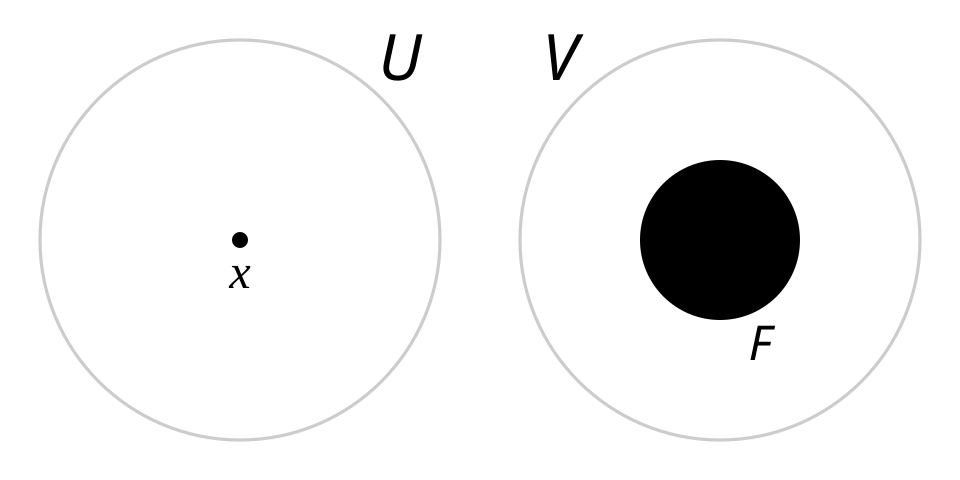
\includegraphics[width=0.9\textwidth]{images/Regular_space.svg.png} % first figure itself
        \caption{regular}
        \label{fig:regular}
    \end{minipage}\hfill
    \begin{minipage}{0.45\textwidth}
        \centering
        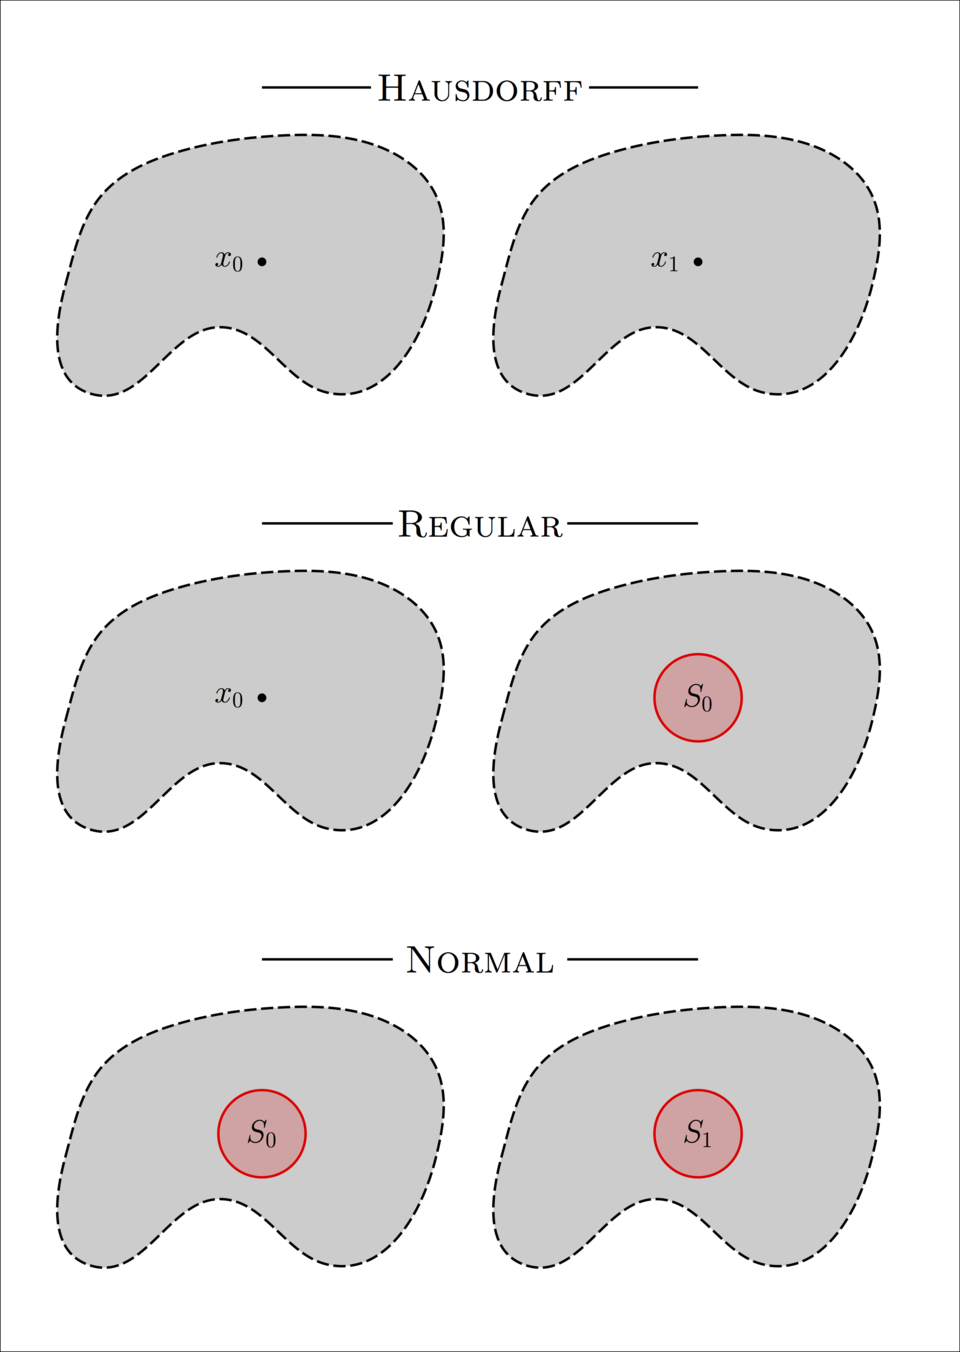
\includegraphics[width=0.9\textwidth]{images/960px-Hausdorff_regular_normal_space_diagram.png} % first figure itself
        \caption{regular, normal and Hausdorff}
        \label{fig:normalregHous}
    \end{minipage}
\end{figure}
% \begin{figure}[ht!]
%     \centering
%     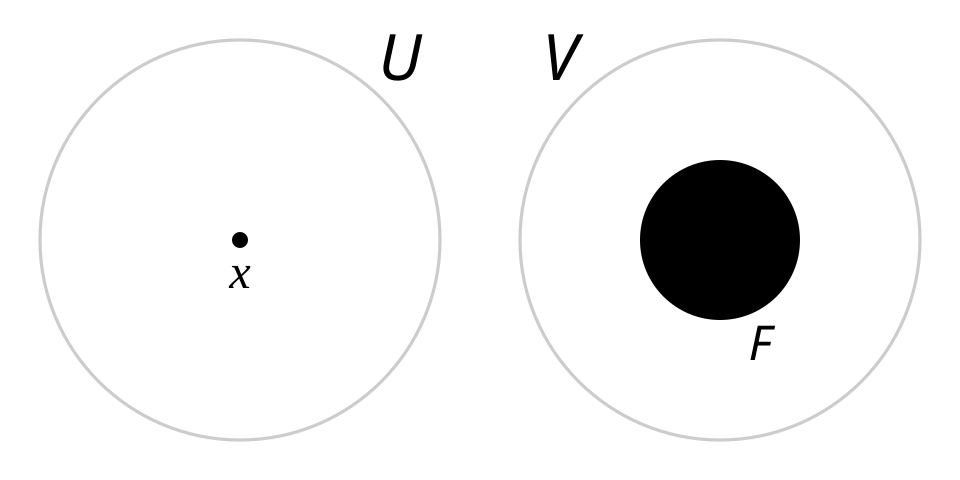
\includegraphics[width=0.9\textwidth]{images/Regular_space.svg.png} % first figure itself
%     \caption{regular}
%     \label{fig:regular}
% \end{figure}
% \begin{figure}[ht!]
%     \centering
%     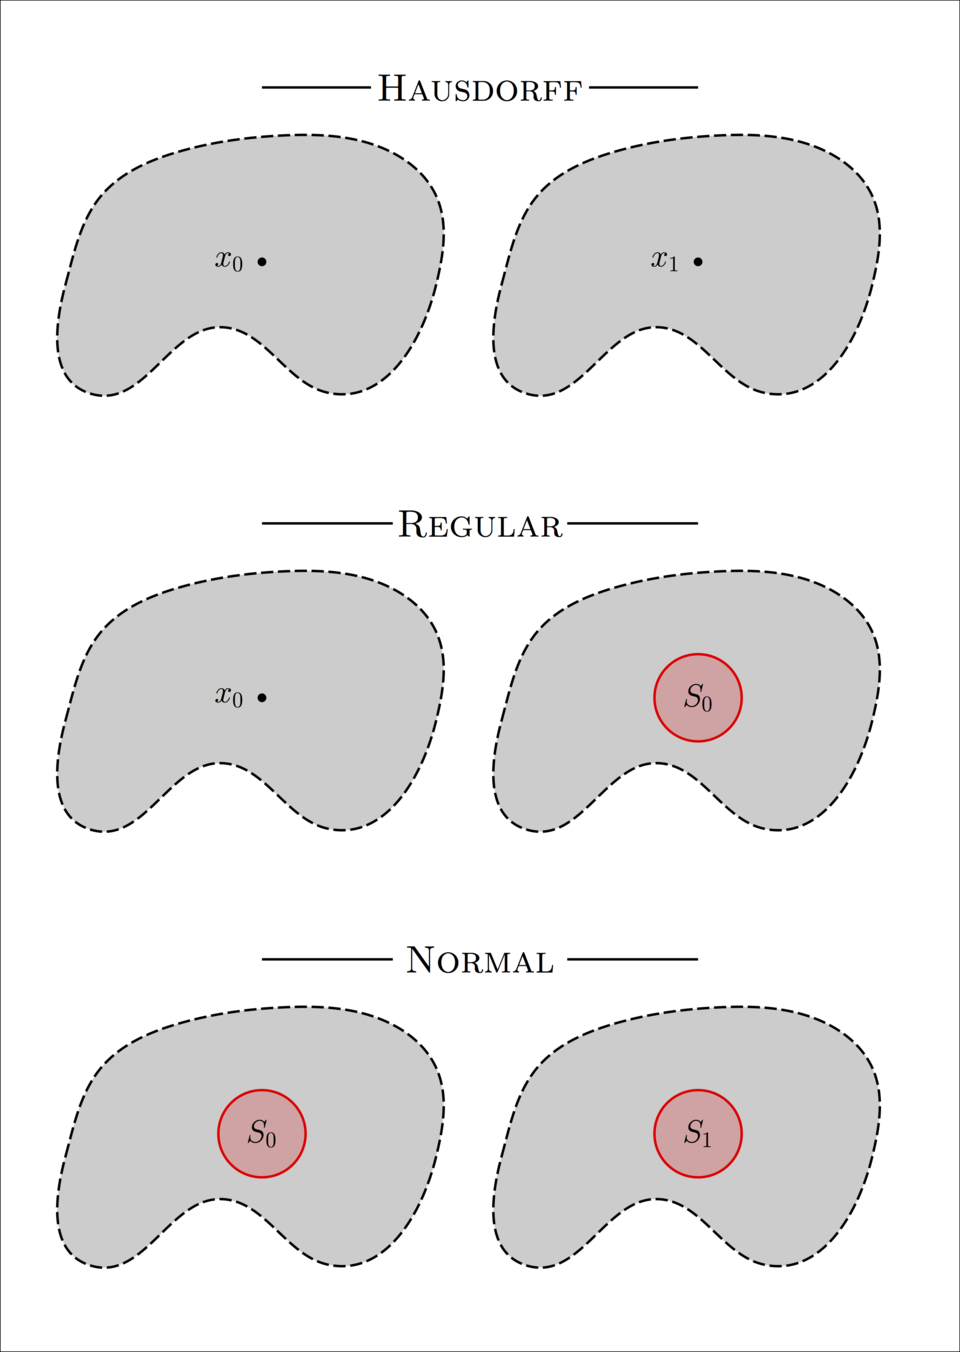
\includegraphics[width=0.9\textwidth]{images/960px-Hausdorff_regular_normal_space_diagram.png} % first figure itself
%     \caption{regular, normal and Hausdorff}
%     \label{fig:normalregHous}
% \end{figure}
% \begin{figure}[ht!]
%     \centering
%     \begin{minipage}{0.45\textwidth}
%         \centering
%         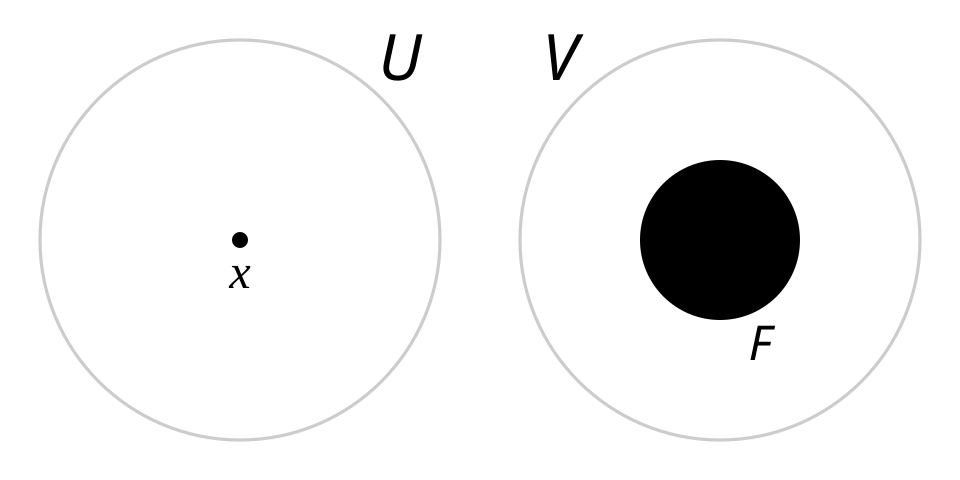
\includegraphics[width=0.9\textwidth]{images/Regular_space.svg.png} % first figure itself
%         \caption{regular}
%         \label{fig:fig1}
%     \end{minipage}\hfill
% \end{figure}
% \begin{figure}[ht!]
%     \centering
%     \begin{minipage}{0.45\textwidth}
%         \centering
%         \includegraphics[width=0.9\textwidth]{figLinearSine1_cbf0039b/draw_2D__GeneredData.png} % first figure itself
%         \caption{$\frac{\sqrt{2}}{2}*sin(x+\frac{\pi}{4})$}
%         \label{fig:fig2}
%     \end{minipage}\hfill
%     \begin{minipage}{0.45\textwidth}
%         \centering
%         \includegraphics[width=0.9\textwidth]{figLinearSine1_cbf0039b/draw_2D__GeneredEqu.png} % second figure itself
%         \caption{$f$ errors}
%     \end{minipage}
% \end{figure}
% \begin{figure}[ht!]
%     \centering
%     \begin{minipage}{0.45\textwidth}
%         \centering
%         \includegraphics[width=0.9\textwidth]{figAugWithP/draw_3D__latentPlot0.png} % first figure itself
%         \caption{first component latent space of $y^\delta(\rho)$}
%         \label{fig:fig3}
%     \end{minipage}\hfill
%     \begin{minipage}{0.45\textwidth}
%         \centering
%         \includegraphics[width=0.9\textwidth]{figAugWithP/draw_3D__latentPlot1.png} % second figure itself
%         \caption{second component latent space of $y^\delta(\rho)$}
%     \end{minipage}
% \end{figure}
% \begin{figure}[ht!]
%     \centering
%     \begin{minipage}{0.45\textwidth}
%         \centering
%         \includegraphics[width=0.9\textwidth]{figAugWithP/draw_2D__circleData.png} % first figure itself
%         \caption{original data $x_\delta$}
%         \label{fig:fig4}
%     \end{minipage}\hfill
%     \begin{minipage}{0.45\textwidth}
%         \centering
%         \includegraphics[width=0.9\textwidth]{figAugWithP/draw_2D__circleGeneInTask.png} % second figure itself
%         \caption{regenerate data $y_\delta$}
%     \end{minipage}
% \end{figure}


% \begin{thebibliography}{99}
%     % Use \bibitem to reference your sources. Example:
%     \bibitem{example-ref} Author Name, \textit{Title of the Paper}, Journal, Year.
% \end{thebibliography}
\bibliographystyle{plain}  % or another style like unsrt, IEEEtran, etc.
\bibliography{references}  % references.bib is the file name

\end{document}
